\section{Hamiltonian for Max-Cut}
\SectionPage{}

\begin{frame}{Max-Cut}
\begin{center}
    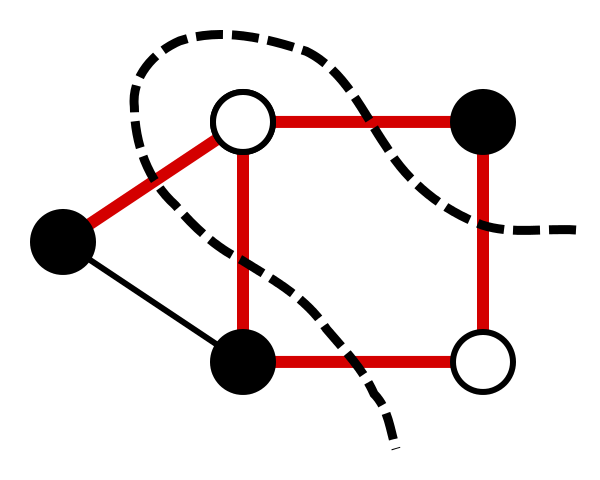
\includegraphics[width=0.5\textwidth]{img/lec6/Max-cut.svg.png}
\end{center}
\begin{itemize}
    \item one variable \( s_i \) per vertex
    \item \(s_i\) can take values \( -1, +1 \) 
\end{itemize}
\[ \text{MaxCut}(s_1, ..., s_n) = \max\frac{1}{2} \sum\limits_{(s_i, s_j) \in E} (1 - s_i s_j) \]
\end{frame}

\begin{frame}{Hamiltonian for MaxCut}
\begin{align*}
    \text{MaxCut}(s_1, ..., s_n) 
    & = \max\frac{1}{2} \sum\limits_{(s_i, s_j) \in E} (1 - s_i s_j) \\
    & = \max\frac{1}{2} \sum\limits_{(s_i, s_j) \in E} (- s_i s_j) + \text{const} \\
    & \equiv \max\sum\limits_{(s_i, s_j) \in E} (- s_i s_j) \\
    & \equiv \min\sum\limits_{(s_i, s_j) \in E} s_i s_j
\end{align*}
\end{frame}

\begin{frame}{Hamiltonian for MaxCut}
Map \(s_i\) to an operator that has 
\begin{itemize}
    \item eigenvalue \(+1\) associated to \(\ket{0}\);
    \item eigenvalue \(-1\) associated to \(\ket{1}\);
\end{itemize}

This operator is \(Z\). \bigskip

\[ H = \sum\limits_{(s_i, s_j) \in E} Z_i Z_j \]

\alert{Your turn}: create the Hamiltonian analytically for graph having vertexes \(V = \{v_1, v_2, v_3\}\) and edges \(E=\{(v_1, v_2); (v_2, v_3)\}\). 

\begin{center}
    \begin{tikzpicture}
    \node (v1) at (0,0) {\(v_1\)};
    \node (v2) at (1,1) {\(v_2\)};
    \node (v3) at (2,0) {\(v_3\)};
    \draw (v1) -- (v2) -- (v3);
    \end{tikzpicture}
\end{center}

\end{frame}

\begin{frame}[fragile]{Hamiltonian for MaxCut}
\begin{minted}{python}
import numpy as np
Z = np.array([[1, 0], [0, -1]])
I = np.array([[1, 0], [0, 1]])
H = np.kron(np.kron(Z, Z), I) # Z_1 Z_2
H += np.kron(I, np.kron(Z, Z)) # Z_2 Z_3
# array([[ 2,  0,  0,  0,  0,  0,  0,  0],
#        [ 0,  0,  0,  0,  0,  0,  0,  0],
#        [ 0,  0, -2,  0,  0,  0,  0,  0],
#        [ 0,  0,  0,  0,  0,  0,  0,  0],
#        [ 0,  0,  0,  0,  0,  0,  0,  0],
#        [ 0,  0,  0,  0,  0, -2,  0,  0],
#        [ 0,  0,  0,  0,  0,  0,  0,  0],
#        [ 0,  0,  0,  0,  0,  0,  0,  2]])
\end{minted}

Solution associated to \(\ket{010}\), \(\ket{101}\) has minimum valued eigenvalues.
\end{frame}